\cotefile{13}
\scanpage{38}
% The writing is turned 180 degrees in the scan.
\[
\begin{aligned}
G'_{K} \quad P \qquad G_{K} &\qquad G_{\mathbb{C}} / \mathbb{C} \\
                            &\qquad G / \unsure{\mathbb{Q}|Q}
\end{aligned}
\]

\unsure{,|1|)}

% Paper watermark, sideways and mirrored relative to the manuscript; two lines.
\noindent\textsc{Extra Strong}\\
\unsure{Maunoury|Marmury|Maimury} 1808
% archive sheet number: 37
\scanpage{39}
Nous allons introduire une autre structure de nature \unsure{transcendante}, en introduisant le \unsure{rev.|ver.} universel $\bar S_{\mathbb C}$ de $S(\mathbb C)$ en $\xi$ $\unsure{\xi|:}$ [sous-entendu : de la comp. connexe de $\xi$ dans $S(\mathbb C)$].

Soit $\unsure{\gamma|\mathscr{Y}}_{G}$ l'ensemble des hom. de $\unsure{\mathbb S|S}=\prod_{\mathbb C/\mathbb R}\mathbb G_{m\,\mathbb C}$ dans $G_{\mathbb R}$, correspondant à l'hom central \deleted{\unsure{donné}} $i:\mathbb G_m \unsure{\relbar|\longrightarrow} G$ donné par $i(\lambda)=i_1(\lambda)i_2(\lambda)$. \margin{\rule{0.35pt}{2.1\baselineskip}}On considère $\gamma$ comme variété \deleted{\unsure{an.|anal.}} holomorphe où \deleted{$\unsure{\gamma|G}$} $G(\mathbb R)$ et à fortiori $G(\unsure{\mathbb Q|Q})$ opère. Ceci \unsure{posé|fait}, on a une \uline{application}
\[
\boxed{f:\bar S_{\mathbb C}\longrightarrow\gamma_G}
\]
satisfaisant les conditions

\uline{12)}\unsure{a.|.} \ a) $f(\bar\xi\inserted{\text{le pt marqué de }\bar S_{\mathbb C}})={}\text{l'hom }\mathbb S\unsure{\relbar|\longrightarrow} G_{\mathbb R}$ défini par $i_1^{\mathbb C},i_2^{\mathbb C}$ de c).

b) $f(g\bar s)=\unsure{w_{1}|w|h_{1}|h_{\gamma}|\rho_{1}|\rho_{\gamma}}(g)f(\bar s)$ si $g\in\pi_1(S(\mathbb C),\xi),\ \bar s\in\bar S_{\mathbb C}$

c) $f$ est \uline{holomorphe}.

\unsure{14)|15)} (Moyennant Hodge) \deleted{Pour tout $\bar s\in\bar S_{\mathbb C}$, le plus grand sous-groupe algébrique de $G$ qui sur $\mathbb R$ contient $f(\bar s)(\mathbb S)\subset G_{\mathbb R}$, et qui de plus contient $H$} \inserted{Le composé \deleted{\unsure{de}} $\bar S_{\mathbb C}\longrightarrow\gamma_G\longrightarrow\gamma_{\widetilde G}$} (qui à priori \inserted{\unsure{vû|vu|n\textsuperscript{o}} : 12 b)} se factorise par \deleted{\unsure{$\bar S_{\mathbb C}$}} $S(\mathbb C)^{\unsure{\circ|0}}$) est une application \uline{constante}.

13) Si $\bar s\in\bar S_{\mathbb C}$ se trouve sur le point $t$ de $S$ [il nous \unsure{plaît|plait|suffit} bien que $P$ comme torseur à connexion \unsure{intégr.} $P_S$ soit défini sur $S$] de sorte qu'on a torseur à conn. intégrable \deleted{\illegible{1}} $(P_t,G_{k(t)})$ sur $k(t)$, \deleted{\unsure{soit}} l'hom $f(\bar s)_{\mathbb C}:\mathbb S_{\mathbb C}\longrightarrow(G_{k(t)})_{\mathbb C}\simeq G_{\mathbb C}$ [définissant une bigraduation\inserted{ donc filtration} sur le foncteur $T_{\mathbb C}$, $T$ foncteur oubli sur les $G$-modules] est \uline{compatible} avec le torseur $P_t$ sous $G_{k(t)}$ et sa $\unsure{C|\mathbb C|G}$-trivialisation $p(\bar s)$ [$p:\bar S_{\mathbb C}\longrightarrow(P_S)_{\mathbb C}$ $\unsure{\in|\epsilon}$ ici est \unsure{le|la} $S(\mathbb C)^{\circ}$-morphisme \unsure{caractérisé} par la condition que $p(\bar\xi)=\alpha$].
% archive sheet number: 38
\scanpage{40}
\unsure{10)|19)} (Modulo conjecture de Hodge) $G^{\unsure{\circ|0}}$ est engendré sur $\unsure{\mathbb Q|Q}$ par $i_1^{\mathbb C}$.

\deleted{\unsure{10)} $G$}

% slanted
\margin{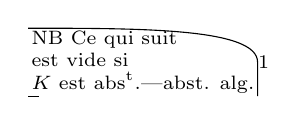
\begin{tikzpicture}[baseline=(current bounding box.north),font=\scriptsize]
\node[align=left,inner sep=1pt] (note) {\uline{NB} Ce qui suit\\est vide si\\$K$ est \unsure{abs\textsuperscript{t}.|abst.} alg.};
\draw (note.north west) .. controls (note.north) and (note.north east) .. (note.east)
.. controls (note.east) and (note.south east) .. (note.south east);
\draw (note.south west) -- ([xshift=4pt]note.south west);
\node[anchor=west,inner sep=0pt] at (note.east) {\deleted{\illegible{1}}};
\end{tikzpicture}}
Soit $R\subset G$ le sous groupe algébrique engendré par $\unsure{w|u|\omega}(\pi_1(S(\mathbb C),\xi))$. Il est \uline{invariant} moyennant \unsure{9)|4)} [car l'image fermée de $\pi_1(S(\mathbb C),\unsure{\xi|1})\unsure{\relbar|\longrightarrow}\pi_1(S,\xi)$\unsure{\}|,} est un sous-groupe invariant\unsure{\}|,}, le quotient étant $\pi_1(\operatorname{Spec} k,\xi)$, où $k$ est la clôture alg. de $\mathbb Q$ dans $K$]. \deleted{\unsure{Le|La} \unsure{composé}} En vertu de 4), l'hom.
\diagram{\begin{tikzcd}[ampersand replacement=\&,column sep=1.4em,row sep=.5ex]
{} \& {} \& \inserted{\widetilde G(\mathcal A),\ \text{où }\widetilde G=G/R,}\\
\pi_1(S\unsure{\mathbb C|\in},\xi) \arrow[r] \& G(\unsure{\mathcal A|\mathscr A|A}) \arrow[ur] \& {}
\end{tikzcd}}
se factorise donc en
\[
\tilde u:\underset{\substack{\Vert\\[-.4ex]\simeq\\[-.4ex]\unsure{\pi_1|\Vert}}}{\pi_1(\operatorname{Spec}(k),\xi)}
\longrightarrow\widetilde G(\mathcal A)
\]

D'autre part, on considère le torseur $\widetilde P=P/R$ sous $\widetilde G$, avec la connexion intégrable déduite de celle de $P$. On a

\margin{\deleted{\uline{\illegible{1}}}}
\unsure{16)|18)|10)} \inserted{(Modulo Hodge)} $(\widetilde P,\widetilde G)$ avec sa connexion intégrable ``se descend à $k$'', donc on a un torseur $(\widetilde P_0,(\widetilde G/k))$ sur $k$, et un isom de torseurs
\begingroup
\csname tagsleft@true\endcsname
\[
\widetilde P=P/R\simeq\widetilde P_0\otimes_k K \tag*{(*)}
\]
\endgroup

\deleted{De plus, \deleted{\unsure{posant}} introduisant $R'\subset G'$ correspondant à $R$, et $\widetilde G'=G'/R'$, de sorte qu'on a un isom}
\[
\deleted{\widetilde G'=\widetilde G'_0\otimes_k K,\qquad
\widetilde G'_0=\underline{\operatorname{Aut}}_{(\widetilde G/k)-}(\widetilde P_0),}
\]
\deleted{le ss-groupe \deleted{$\unsure{\widetilde H'|H'}\subset\unsure{\widetilde G'|G'}$} \inserted{$\widetilde H'=H'/H'\cap R'\unsure{=|\simeq}\operatorname{Im}(H'\longrightarrow\widetilde G')$} est ``défini sur $k$'' i.e. provient de $\widetilde H'_0\subset\widetilde G'_0$}

\inserted{Enfin l'isom \unsure{(*)|ci}, $\unsure{\in|\xi}$ qui} \deleted{La structure de filtration sur le foncteur $T$} définit, pour un $\widetilde G$-module $M$, une structure de descente sur $P\mathbin{\times}^{G_K}M_K$ à $k$\unsure{,|;} [c'est celle définie par la connexion intégrable de $P\mathbin{\unsure{\alpha|\times}}^{G_K}M_K$], donne une donnée de descente \uline{compatible} avec la filtration, i.e cette dernière est \uline{horizontale}, $\bigl[\!\bigl[$ donc \deleted{\illegible{1}} $\widetilde H'=\operatorname{Im}(H'\longrightarrow\widetilde G')$, $\widetilde Q\unsure{,|_{,}}=Q\mathbin{\times}^{\unsure{H'|\widetilde H'}}\widetilde H'$, se descendent \unsure{respect\textsuperscript{t}|respectiv\textsuperscript{t}} en $\widetilde H'_0\subset\widetilde G'$ et un torseur à droite $Q_0$ sous $\widetilde H'_0$, \deleted{\unsure{et}} (d'où $\widetilde H''_0$ et $\widetilde G''_0$ qui descendent $H''$ et $\widetilde G''$), et \deleted{\unsure{après}} les composés $\tilde i_1,\tilde i_2:\mathbb G_m\underset K{\longrightarrow}G''\longrightarrow\widetilde G''$ se descendent en $(\tilde i_1)_0,(\tilde i_2)_0:\mathbb G_{m\,k}\longrightarrow\widetilde G''_0$ $\bigr]\!\bigr]$.
% archive sheet number: 39
\scanpage{41}
$S$ schéma régulier connexe de \unsure{t.f.|s.t.f.} sur $\unsure{\mathbb Q|Q}$

$k$ clôture alg. de $\mathbb Q$ dans $\Gamma(S,\unsure{\mathscr O|\mathcal O}_S)$, de sorte que $k/\mathbb Q$ \unsure{fini|finie}, $S/k$ géom. \unsure{conn|conn.}

$k\hookrightarrow\mathbb C$ une immersion

$\unsure{\mathcal M|\mathscr M}$ catégorie de motifs (``iso'', lisses $\frac12$ simples) sur $S$, $\mathcal M$ de type fini.

L'immersion $k\hookrightarrow\mathbb C$ définit une classe d'isomorphie de foncteurs fibres\inserted{ \unsure{val}\,/\,$\mathbb Q$} sur $\mathcal M$, savoir les $T_{\xi}\deleted{\unsure{T|P}}:M\longrightarrow T_B(M_{\xi}),\quad \xi\in S(\mathbb C)$\inserted{$\underset{\deleted{\operatorname{Hom}_k(\operatorname{Spec}\mathbb C,S)}}{\Vert}$}.

Soit \deleted{$G$ un groupe alg. /$\mathbb Q$ (réductif) isomorphe aux $\underline{\operatorname{Aut}}_{\otimes}(T_{\xi})$\unsure{en|.}.} \inserted{$T$ un foncteur fibre de cette classe, et \deleted{\unsure{soit}}}
\[
G=\underline{\operatorname{Aut}}_{\otimes}(T),\quad\text{donc }\mathcal M\approxeq\operatorname{Rep}(G)
\]

Alors
\[
P=\underline{\operatorname{Isom}}_{\otimes}(T_S,T_{\mathrm{DR}})
\]
est un torseur sous $G_S$. Il est muni d'une \uline{connexion} intégrable relativement à $k$ (ou $\mathbb Q$, c'est kif kif) compatible avec $G$\unsure{,|.}

De plus le foncteur $T_{\mathrm{DR}}$, isomorphe par construction de $P$ à
\[
M\longmapsto P\mathbin{\times}^{G_S}M_S\qquad\text{sur }\operatorname{Rep}(G)
\]
est muni d'une $\otimes$-\uline{filtration}

\deleted{\unsure{Soit} $S_{\mathbb C}$} Considérons $S(\mathbb C)$, et le revêtement $\deleted{\bar S}\unsure{\widetilde P|\bar P}_{\mathbb C}$ de $S(\mathbb C)$ dont la fibre en $\xi\in S(\mathbb C)$ est formée des isom $T\longrightarrow T_{\xi}$. Alors $\bar S_{\mathbb C}$ est un revêtement principal de $S(\mathbb C)$, de groupe $G(\mathbb Q)$, \deleted{qui n'est autre que le rev. \unsure{associé}, \unsure{fibré} \unsure{pr.} assoc. à $P_{\mathbb C}^{\mathrm{an}}$ sur $S_{\mathbb C}^{\mathrm{an}}\underset{S(\mathbb C)}{\Vert}$} et \unsure{un|on} \deleted{\unsure{une}} \deleted{\unsure{avec|de} $S_{\mathbb C}$} \deleted{\unsure{application}} \inserted{morphisme (hol)} évident
\[
p:\deleted{\unsure{\bar S|\bar P}}\widetilde P_{\mathbb C}
\longrightarrow P_{\mathbb C}^{\mathrm{an}}\deleted{\unsure{G|g}}
\]
satisfaisant
\[
\left[\begin{aligned}
&p(\unsure{\xi|g}\,x\,g)=p(x)g\\
&p\ \text{compatible aux connexions \unsure{sur un|sur nos|sur}}\\
&\hspace{4em}S\text{-fibrés}\ldots
\end{aligned}\right.
\]

\[
\deleted{f:\bar S_{\mathbb C}\unsure{\relbar|\longrightarrow}\unsure{\gamma|\mathscr Y}_{G}}
\]
\deleted{où $\gamma_G$ est l'espace des structures de Hodge sur $G_{\mathbb R}$ (compatibles, si on y tient, avec un $i:\mathbb G_m\unsure{\relbar|\longrightarrow} G$ fixé). Alors $f$ satisfait aux conditions}

\deleted{a) $f$ holomorphe}

\deleted{b) $f(xg)=g^{-1}f(x)$ pour $g\in G(\mathbb Q)$ [\uline{NB} $G(\mathbb R)$ donc $G(\mathbb Q)$ opère sur $\gamma_G$ par autom. \unsure{intérieurs|intégrieurs},]}

\deleted{c) .}
% archive sheet number: 40
\scanpage{42}
Lorsqu'on se fixe un point $\xi_0\in S(\mathbb{C})$,\deleted{\unsure{$\xi$|,}}\inserted{et qu'on prend $T=T_{\xi_0}$,} alors la donnée du revêtement principal $\bar S_{\mathbb{C}}$ et de $\deleted{\unsure{f|p}}\unsure{p|f}$ équivaut à la donnée de
\[
\begin{aligned}
&\deleted{\unsure{w(\pi_1(S(\mathbb{C}),\xi_0)|w:\pi_1(S(\mathbb{C}),\xi_0)}}\\
&\unsure{w|\omega}:\pi_1(S(\mathbb{C}),\xi_0)\longrightarrow G(\mathbb{Q})\subset G(\mathbb{C})
\end{aligned}
\]
[il est associé à la connexion intégrable de $P$, qui en définit une sur $P_{\mathbb{C}}^{\mathrm{an}}$ sur $S_{\mathbb{C}}^{\mathrm{an}}$, d'où $\Gamma=\pi_1(S(\mathbb{C}),\xi_0)\longrightarrow G(\mathbb{C})$, dont il faut demander qu'il se factorise par $G(\mathbb{Q})$] et à un \deleted{\unsure{hom|hom.} du revêtement universel} point $\alpha_0$ de $P(\xi_0)$ i.e. une trivialisation de $P_{\xi_0}$, qui définit alors un unique morphisme \inserted{$q$} du rev. universel $\bar S_{\mathbb{C}}$ de $S_{\mathbb{C}}$ dans $P_{\mathbb{C}}^{\mathrm{an}}=P(\mathbb{C})$, appliquant le pt marqué $\bar\xi_0$ en $\alpha_0$ ; il satisfait \deleted{\unsure{à|la}} $q(\bar s\gamma)=q(\bar s)w(\gamma)$ pour tout $\unsure{\hat s|\bar s}\in\bar S_{\mathbb{C}}$, \deleted{$\unsure{\gamma\in\pi_1(S|\gamma\in\pi_1}$} $\gamma\in\pi_1(S(\mathbb{C}),\xi_0)$, \deleted{Le morphisme \unsure{satisfai|satisfait}} et définit
\[
\widetilde P_{\mathbb{C}}=\overline{\unsure{S|\mathbb{S}}}_{\mathbb{C}}\mathbin{\times}^{\Gamma}G(\mathbb{Q})\hookrightarrow P_{\mathbb{C}}^{\mathrm{an}}
\]
[\unsure{restriction|restiction} du groupe structural \inserted{du $P_{\mathbb{C}}^{\mathrm{an}}$} de $G(\mathbb{C})$ à $G(\mathbb{Q})$].

Comme structure importante, il y a une application
\[
f:\widetilde P_{\mathbb{C}}\unsure{\relbar|\longrightarrow}\unsure{\gamma|\mathscr{Y}}_G
\]
où $\gamma_G$ est l'ens. des structures de Hodge sur $G_{\mathbb{R}}$ (\deleted{\unsure{associées|associés},}\inserted{compatibles,} si on y tient, avec un morphisme $i:\unsure{\mathbb{G}|G}_{m\,\mathbb{Q}}\unsure{\longrightarrow|\relbar}G$ donné). Cette application $f$ satisfait les conditions

a) $f$ holomorphe

b) $f(xg)=g^{-1}f(x)$ \qquad $g\in G(\mathbb{Q}),\,x\in\widetilde P_{\mathbb{C}}$

\unsure{b|c}) $\forall x\in\widetilde P_{\mathbb{C}}$ sur le point $s$ de $S$, la \inserted{structure de} filtration sur $T_{\mathbb{C}}$ sur $\operatorname{Rep}(G)$, définie par $f(\unsure{x|s}):\mathbb{S}\longrightarrow G_{\mathbb{R}}$, est compatible
% archive sheet number: 41
\scanpage{43}
avec le torseur $P_s$ sous $G_{k(s)}$ et la trivialisation $p(x)\in P_s(\mathbb{C})$.

En termes de $\unsure{w|\omega}$ et $q:\bar S_{\mathbb{C}}\longrightarrow P_{\mathbb{C}}^{\mathrm{an}}$, la donnée de $f$ revient à la donnée de
\[
f:\bar S_{\mathbb{C}}\longrightarrow\unsure{\gamma|\mathscr{Y}}_G
\]
satisfaisant les conditions

a) $f$ holomorphe

b) $f(xg)=w(g)^{-1}f(x)$

c) \deleted{$\unsure{f(\xi_0)|f(\bar\xi_0)}$} $\forall\bar s\in\bar S_{\mathbb{C}}$, \inserted{sur $s\in S$} $f(\bar s):\mathbb{S}\unsure{\relbar|\longrightarrow}G_{\mathbb{R}}$ est compatible avec le torseur $P_s$ sur $G_{k(s)}$ et sa trivialisation $q(x)\in P_s(\mathbb{C})$.

Enfin, \deleted{pour tout $\unsure{k|\ell}$}, on se donne une ``\unsure{restiction|restriction}'' du rev. $\widetilde{\unsure{P|\mathbb P}}_{\mathbb{C}}\mathbin{\times}^{G(\mathbb{Q})}G(\unsure{\mathcal A|\mathscr A})\deleted{\unsure{\mathbb{Q}_{\ell}|\mathbb{Q}_l}}$ sur $S_{\mathbb{C}}^{\mathrm{an}}$ en un revêtement
% slanted
\margin{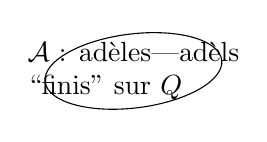
\begin{tikzpicture}[baseline=(current bounding box.center)]
\node[inner sep=0pt,align=left] (note) {$\mathcal A$ : \unsure{adèles|adèls}\\``finis'' sur $\mathbb{Q}$};
\draw[rotate around={7:(note.center)}] (note.center) ellipse [x radius=1.13cm,y radius=.47cm];
\end{tikzpicture}}
\deleted{sur $S$ \unsure{dont|de} \unsure{le|de} \unsure{gpe|grp} $\unsure{G_\ell|G_{\mathbb{Q}_\ell}}$} de groupe $G(\mathbb{Q}_{\ell})$ sur $S$, En termes \inserted{de $\xi_0$ et} de $\Gamma=\pi_1(S(\mathbb{C}),\unsure{\xi|\mathord{)}}_0)$, on se donne une factorisation de $\Gamma\xrightarrow{w}G(\mathbb{Q})\unsure{\longrightarrow|\relbar}G(\mathcal A)$ par $\Gamma\longrightarrow\pi_1\underset{\substack{\Vert\\\pi_1}}{(S},\xi_0)\longrightarrow G(\mathcal A)$. Quant au revêtement $\widetilde P_{\mathbb{C}}\mathbin{\times}^{G(\mathbb{Q})}(\deleted{\unsure{G|\mathcal A}}\unsure{\mathcal A|G}/G^{\unsure{0|\circ}})(\mathcal A)$, \deleted{\unsure{égal à|égale à} $\widetilde P_{\mathbb{C}}\times$}\inserted{il est} associé à $\widetilde P_{\mathbb{C}}/G^0(\mathbb{Q})\deleted{\unsure{\text{de}|\text{du}}}\unsure{=|\relbar}(P/G^0)_{\mathbb{C}}^{\mathrm{an}}$, \deleted{\unsure{qui|qu'}}\unsure{est|et} \unsure{à|:} \unsure{ce|en} \unsure{titre} \unsure{leur|leurs} restriction à $S$ \deleted{\unsure{est|et}} est connue. \unsure{On veut|On voit|Bien voir} que ce \unsure{soit|sont} \unsure{celle|celles} \unsure{donnée|données} plus haut\unsure{.....|....}

\deleted{\uline{NB} \unsure{L'application|l'application} $f$ \unsure{est|et}}
% archive sheet number: 42
\scanpage{44}
A) Groupe algébrique \deleted{\unsure{$G$|le}}\unsure{[|(}réductif\unsure{]|)} $G$ sur $\mathbb{Q}$

B) \unsure{fibré|fibre} principal à connexion intégrable $\unsure{P|\mathbb P}$ \unsure{sous|sur} $G_S$

% slanted; marginal brace extends alongside C) and D)
\margin{\begin{tikzpicture}[x=1cm,y=1cm,baseline=(current bounding box.north)]
\node[anchor=north east,inner sep=1pt] at (-.09,0) {\unsure{où|ou} $q,f'$};
\draw (.03,0) .. controls (-.04,-.35) and (.23,-1.10) .. (-.09,-1.24)
.. controls (.13,-1.33) and (.14,-2.05) .. (.15,-2.48);
\end{tikzpicture}}
C) Restriction du groupe $G_{\mathbb{C}}^{\mathrm{an}}$ à $G(\mathbb{Q})$ dans $P_{\mathbb{C}}^{\mathrm{an}}$, d'où
\diagram{\begin{tikzcd}[ampersand replacement=\&,column sep=2em]
\text{rev.}\quad\deleted{\unsure{\bar S|\widetilde S}}\quad\widetilde P \arrow[r,hook,"p"] \& P_{\mathbb{C}}^{\mathrm{an}} \arrow[r] \& P
\end{tikzcd}}

D) Application holomorphe
\[
f:\widetilde P\unsure{\longrightarrow|\relbar}\unsure{\gamma|\mathscr{Y}}_G
\]
satisfaisant $f(xg)=g^{-1}f(x)$ $(x\in\widetilde P,\,g\in G(\mathbb{Q})$ et compatible avec les données B) et $p$ de C).

E) Restriction de $\widetilde P\mathbin{\times}^{G(\mathbb{Q})}G(\unsure{\mathcal A|\mathscr A})$ à $S$, avec compatibilité relativement à $G/G^{\unsure{0|\circ}}$.

NB La connaissance de A) B) C) et de $f(\xi_0)$, où $\xi_0\in\widetilde P$ est au dessus du point générique de $S$ [\uline{\unsure{Condition|condition}} peut-\uline{être superflue}] \margin{??}doit en principe permettre de \unsure{réconstituer|reconstituer} D) tout entier et E) [lorsqu'on sait \deleted{que} que les données proviennent d'une cat. de motifs $M$].

% slanted; boxed marginal note
\margin{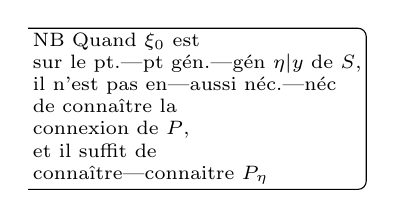
\begin{tikzpicture}[baseline=(current bounding box.north)]
\node[align=left,inner sep=1.5pt,font=\scriptsize] (note) {\uline{NB} Quand $\xi_0$ est\\
sur le \unsure{pt.|pt} \unsure{gén.|gén} $\unsure{\eta|y}$ de $S$,\\
il n'est pas \deleted{\unsure{en|aussi}} \unsure{néc.|néc}\\
de connaître la\\
connexion de $P$,\\
et il suffit de\\
\unsure{connaître|connaitre} $P_{\eta}$};
\draw[rounded corners=3pt] (note.north west) -- (note.north east) -- (note.south east) -- (note.south west);
\end{tikzpicture}}
\uuline{Formule analytique de prolongement de $f$} ?

\uuline{Relations entre D) et E)} ?? [\unsure{Jugendtraum|Jugend traum} ?]
% archive sheet number: 43
